\chapter{Implementation and Technology Stack}\label{chap:implementation}
A variety of technologies were utilized to achieve the underlying results. Simulations were conducted using \textit{PeerSim}, a simulation framework for \textit{Java}. As a result of each simulation, an output file is generated containing different simulation parameters, settings, and performance metrics. The data analysis part of this project is primarily implemented using \textit{Python} as a programming language.

\section{Programming Languages}\label{sec:proglangs}
Python \textit{3.12.6} is used for several tasks, mostly for preparing and analyzing data necessary to conduct simulations and post-simulation analysis. For plotting purposes, \textit{matplotlib v.3.9.1} is used and for handling data and data analysis \textit{scipy v.1.14.1} is used.

For conducting the simulations, \textit{Java Oracle OpenJDK 21.0.1} and \textit{PeerSim v.1.0.5} are used.

\section{Simulation Framwork}\label{sec:simulationframework}
PeerSim is a simulation tool developed in Java, which is composed of two engines: the cycle-driven engine and the event-driven engine. I chose PeerSim for our simulations because it is well-suited for large-scale peer-to-peer simulations. In previous projects, I was able to conduct simulations up to $2^{14}$ nodes and could probably push the boundaries by scaling to even higher dimensions. PeerSim is designed with pluggable components, implemented as interfaces, which are intuitive to use generally. Running a simulation in PeerSim follows four steps. The first step is setting up a \textit{configuration file}, which defines key parameters such as network size and the load-balancing protocols being simulated.

\begin{lstlisting}[caption=Example configuration, captionpos=b, numbers=left, label=lst:exampleConfig]
# network size declaration and initialization
SIZE = 1024
network.size SIZE

# Synchrounous CD Protocol
CYCLES = 100
simulation.cycles CYCLES

# classic PPS protocol definition
protocol.loadBalancingProtocols loadBalancingProtocols.
PushPullSumProtocol
protocol.loadBalancingProtocols.linkable loadBalancingProtocols

# Control classic PPS
control.avgo loadBalancingProtocols.PushPullSumObserver

# The protocol to operate on
control.avgo.protocol loadBalancingProtocols
control.avgo.numberOfCycles CYCLES
\end{lstlisting}

Listing \ref{lst:exampleConfig} shows a section of a configuration file used in this project. This configuration sets up a simulation of the Push-Pull Sum algorithm for a network with 1024 nodes (\textbf{lines 2 and 3}) for 100 rounds (\textbf{lines 6 and 7} in Listing \ref{lst:exampleConfig}). From \textbf{lines 10 to 12}, the Push-Pull Sum algorithm is loaded. The way the algorithms are implemented, one algorithm consists of at least two Java classes, the \textit{<ProtocolName>Protocol.java} and the \textit{<ProtocolName>Observer}, and a shared \textit{loadBalancingParameters}-class, which contains parameters like the cycle counter or topology-specific parameters as depicted in figure \ref{fig:uml}. At \textbf{line 15}, the \textit{control} class is declared, and its usage follows in \textbf{lines 18 and 19}, where it is assigned parameters of type \textit{protocol} and \textit{numberOfCycles}. This process simultaneously handles steps two and three of creating a simulation by selecting the protocols to simulate and specifying control objects. Following that, the last step is to invoke the simulator class \textit{peersim.Simulator.class}. For that, the IDE may be configured to call the simulator class on execution of the program code. Alternatively, a command line in the terminal can also invoke the simulator class. More on this in the PeerSim documentation \cite{peersimdocs}.

PeerSim provides a wide range of classes and interfaces for simulations. In the cycle-driven approach, the framework offers the \textit{CDProtocol} interface, which defines the \textit{nextCycle} method. The \textit{nextCycle} method is executed at the beginning of every simulation round.

Nodes in PeerSim are implemented as containers that hold various protocols. Each node is uniquely identified by a \textit{nodeID} and interacts with the \textit{Linkable} interface, which provides access to neighboring nodes. A class implementing the Linkable interface can override several methods, such as:

\begin{itemize}
    \item \textbf{getNeighbor()}: Retrieves a neighbor with a specified ID.
    \item \textbf{degree()}: Returns the number of connections (or neighbors) a node has.
    \item \textbf{addNeighbor()}: Adds a neighbor to the node's set of neighbors.
\end{itemize}

To monitor or modify simulations, control objects are required. A class implementing the \textit{Control} interface must define the execute method, which can be used to observe or alter the simulation at each round. \cite{peersimdocs}

\begin{figure}
    \centering
    \scalebox{0.45}{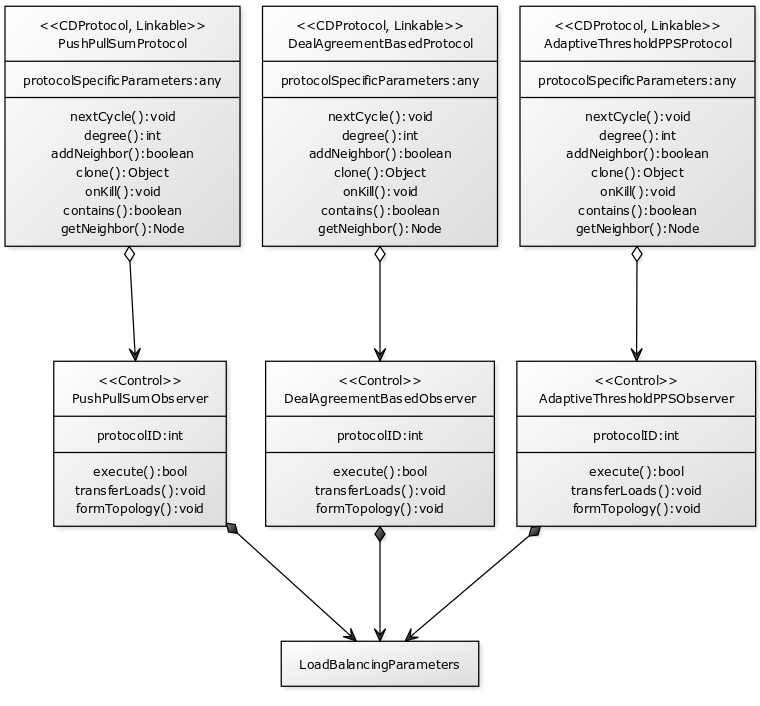
\includegraphics{figures/Diagrams/projectUML.png}}
    \caption{Project structure}
    \label{fig:uml}
\end{figure}

\section{Implementation Details}\label{sec:implementationdetails}
Figure \ref{fig:ProcessModel} depicts a process model, modeling the method chosen to transition from experiment creation to data analysis and visualization. The methodology follows three steps. First, I wrote a Python script that generates configuration files where each node has uniformly distributed random load/sum values. 30 distinct experiments were created to improve statistical significance. Then a Java script reads these configuration files and assigns an initial load value to each node. Then the simulations are conducted. Each simulation outputs a file containing the simulation results, mainly the MSE per round, the loads per round, and the configuration of the network (e.g., which topology is chosen, network size, etc.). The simulation results are averaged per round and then analyzed. Out of the simulation results, plots are generated, showing the MSE reduction per round in log-log or log-linear graphs. Additionally, model-fitting techniques are applied to further analyze trends in the data.

\begin{figure}
    \centering
    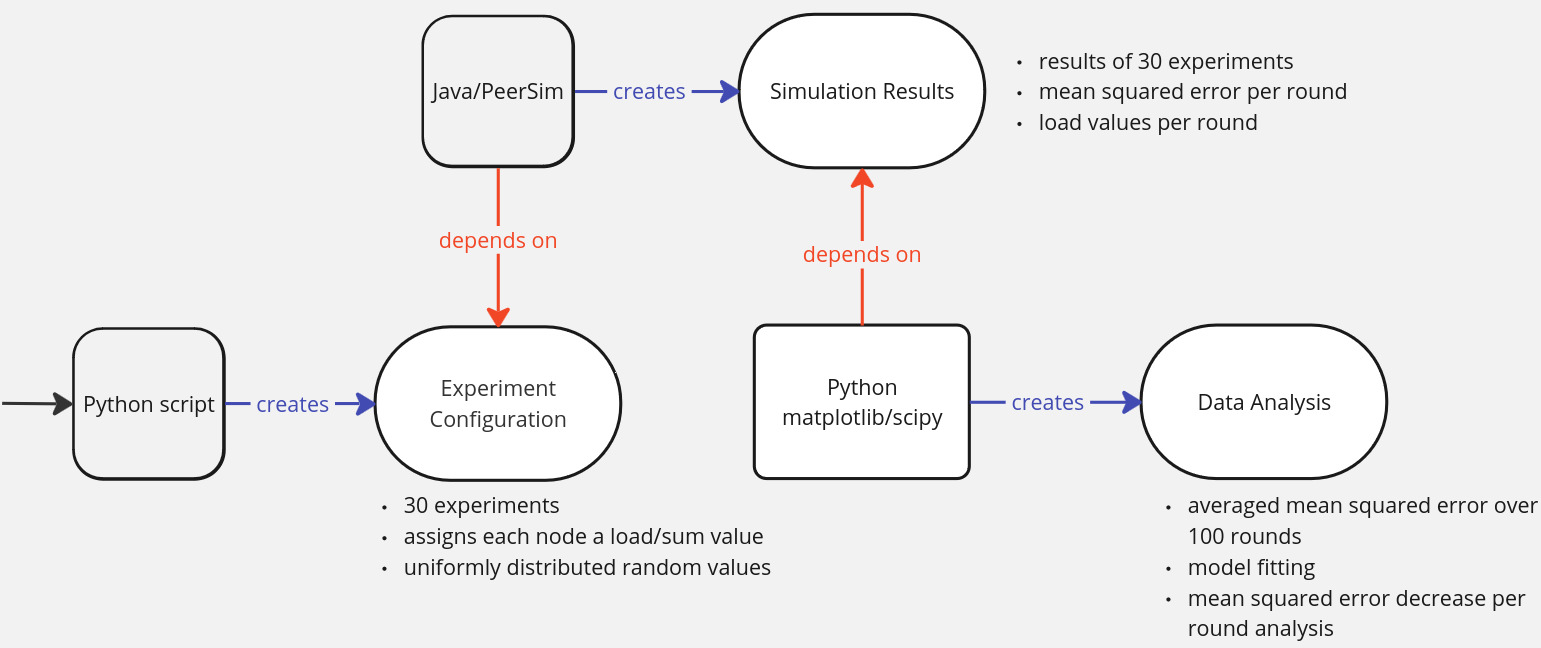
\includegraphics[width=\textwidth]{figures/Diagrams/process_model.png}
    \caption{Process model: methodic}
    \label{fig:ProcessModel}
\end{figure}